% Options for packages loaded elsewhere
\PassOptionsToPackage{unicode}{hyperref}
\PassOptionsToPackage{hyphens}{url}
%
\documentclass[
  12pt,a4paper,lualatex,ja=standard]{bxjsarticle}
\usepackage{lmodern}
\usepackage{amsmath}
\usepackage{ifxetex,ifluatex}
\ifnum 0\ifxetex 1\fi\ifluatex 1\fi=0 % if pdftex
  \usepackage[T1]{fontenc}
  \usepackage[utf8]{inputenc}
  \usepackage{textcomp} % provide euro and other symbols
  \usepackage{amssymb}
\else % if luatex or xetex
  \usepackage{unicode-math}
  \defaultfontfeatures{Scale=MatchLowercase}
  \defaultfontfeatures[\rmfamily]{Ligatures=TeX,Scale=1}
\fi
% Use upquote if available, for straight quotes in verbatim environments
\IfFileExists{upquote.sty}{\usepackage{upquote}}{}
\IfFileExists{microtype.sty}{% use microtype if available
  \usepackage[]{microtype}
  \UseMicrotypeSet[protrusion]{basicmath} % disable protrusion for tt fonts
}{}
\makeatletter
\@ifundefined{KOMAClassName}{% if non-KOMA class
  \IfFileExists{parskip.sty}{%
    \usepackage{parskip}
  }{% else
    \setlength{\parindent}{0pt}
    \setlength{\parskip}{6pt plus 2pt minus 1pt}}
}{% if KOMA class
  \KOMAoptions{parskip=half}}
\makeatother
\usepackage{xcolor}
\IfFileExists{xurl.sty}{\usepackage{xurl}}{} % add URL line breaks if available
\IfFileExists{bookmark.sty}{\usepackage{bookmark}}{\usepackage{hyperref}}
\hypersetup{
  hidelinks,
  pdfcreator={LaTeX via pandoc}}
\urlstyle{same} % disable monospaced font for URLs
\usepackage{graphicx}
\makeatletter
\def\maxwidth{\ifdim\Gin@nat@width>\linewidth\linewidth\else\Gin@nat@width\fi}
\def\maxheight{\ifdim\Gin@nat@height>\textheight\textheight\else\Gin@nat@height\fi}
\makeatother
% Scale images if necessary, so that they will not overflow the page
% margins by default, and it is still possible to overwrite the defaults
% using explicit options in \includegraphics[width, height, ...]{}
\setkeys{Gin}{width=\maxwidth,height=\maxheight,keepaspectratio}
% Set default figure placement to htbp
\makeatletter
\def\fps@figure{htbp}
\makeatother
\setlength{\emergencystretch}{3em} % prevent overfull lines
\providecommand{\tightlist}{%
  \setlength{\itemsep}{0pt}\setlength{\parskip}{0pt}}
\setcounter{secnumdepth}{5}
\usepackage{indentfirst}
\parindent = 1em
\usepackage{dcolumn}
\newcolumntype{.}{D{.}{.}{-1}}
\usepackage{caption}
\captionsetup[table]{name=表}
\captionsetup[figure]{name=図}
\usepackage{hyperref}
\pagestyle{empty}
\usepackage{multicol}
\usepackage{ascmac}
\setpagelayout*{top=10truemm,bottom=30truemm,left=10truemm,right=10truemm}
\usepackage{tikz}
\usetikzlibrary{arrows.meta,decorations,decorations.pathreplacing,arrows}
\usepackage{tabstackengine}
\usepackage{xcolor}
\usepackage{rotating}
\usepackage{txfonts}
\usepackage{fancybox}
\usepackage{dashbox}
\usepackage{tcolorbox}
\tcbuselibrary{theorems,skins}
\usepackage{siunitx}
\usepackage{framed}
\usepackage{enumerate}
\usepackage{lastpage}
\usepackage{pgfplots}
\pgfplotsset{compat=1.15}
\usepackage{mathrsfs}
\ifluatex
  \usepackage{selnolig}  % disable illegal ligatures
\fi

\author{}
\date{\vspace{-2.5em}}

\begin{document}

\renewcommand{\thefootnote}{}
\newcounter{kaunta}
\renewcommand{\thekaunta}{\arabic{kaunta}}
\newcommand{\kaunta}{\refstepcounter{kaunta}%
\thekaunta}
\def\question{\noindent\fbox{\large\makebox[1em]{\text{\kaunta}}} \hspace{1pt}}
\newcounter{skaunta}
\renewcommand{\theskaunta}{\arabic{skaunta}}
\newcommand{\skaunta}{\refstepcounter{skaunta}%
\theskaunta}
\def\squestion{(\text{\skaunta})\hspace{2.5pt}}
\newcommand{\maru}[1]{\raise0.2ex\hbox{\textcircled{\scriptsize{#1}}}}
\newcommand{\jsim}{\mathrel{\text{∽}}}
\newcommand{\jpara}{/\!/}

\newcounter{kcounter}
\setcounter{kcounter}{0}
\newcommand{\kana}{\refstepcounter{kcounter}\ifthenelse{\value{kcounter}=1}{ア}{\ifthenelse{\value{kcounter}=2}{イ}{\ifthenelse{\value{kcounter}=3}{ウ}{\ifthenelse{\value{kcounter}=4}{エ}{\ifthenelse{\value{kcounter}=5}{オ} {\ifthenelse{\value{kcounter}=6}{カ}{\ifthenelse{\value{kcounter}=7}{キ}{\ifthenelse{\value{kcounter}=8}{ク}{\ifthenelse{\value{kcounter}=9}{ケ}{\ifthenelse{\value{kcounter}=10}{コ}{\ifthenelse{\value{kcounter}=11}{サ}{\ifthenelse{\value{kcounter}=12}{シ}{\ifthenelse{\value{kcounter}=13}{ス}{\ifthenelse{\value{kcounter}=14}{セ}{\ifthenelse{\value{kcounter}=15}{ソ}{\ifthenelse{\value{kcounter}=16}{タ}{\ifthenelse{\value{kcounter}=17}{チ}{\ifthenelse{\value{kcounter}=18}{ツ}{\ifthenelse{\value{kcounter}=19}{テ}{\ifthenelse{\value{kcounter}=20}{ト}{\ifthenelse{\value{kcounter}=21}{ナ}{\ifthenelse{\value{kcounter}=22}{二}{\ifthenelse{\value{kcounter}=23}{ヌ}{\ifthenelse{\value{kcounter}=24}{ネ}{\ifthenelse{\value{kcounter}=25}{ノ}{\ifthenelse{\value{kcounter}=26}{ハ}{\ifthenelse{\value{kcounter}=27}{ヒ}{\ifthenelse{\value{kcounter}=28}{フ}{\ifthenelse{\value{kcounter}=29}{ヘ}{\ifthenelse{\value{kcounter}=30}{ホ}{\ifthenelse{\value{kcounter}=31}{マ}{\ifthenelse{\value{kcounter}=32}{ミ}{\ifthenelse{\value{kcounter}=33}{ム}{\ifthenelse{\value{kcounter}=34}{メ}{\ifthenelse{\value{kcounter}=35}{モ}{\ifthenelse{\value{kcounter}=36}{ヤ}{\ifthenelse{\value{kcounter}=37}{ユ}{\ifthenelse{\value{kcounter}=38}{ヨ}{\ifthenelse{\value{kcounter}=39}{ラ}{\ifthenelse{\value{kcounter}=40}{リ}{\ifthenelse{\value{kcounter}=41}{ル}{\ifthenelse{\value{kcounter}=42}{レ}{\ifthenelse{\value{kcounter}=43}{ロ}{\ifthenelse{\value{kcounter}=44}{ワ}{・}}}}}}}}}}}}}}}}}}}}}}}}}}}}}}}}}}}}}}}}}}}}}

\newcommand{\kuran}[1]{\framebox[1.5cm][c]{\maru{#1}}}

\newcommand{\degre}{\ensuremath{^\circ}}

\makeatletter
\newenvironment{figurehere}{\def\@captype{figure}}{}
\makeatother

\newcommand{\haiten}[1]{%
\begin{flushright}%
\footnotesize{<#1>}%
\end{flushright}%
}

\newgeometry{top=10truemm,bottom=10truemm,left=20truemm,right=20truemm}

\thispagestyle{empty}
\begin{center}
\phantom{empty}

\vspace{60truemm}

\hspace{4em} {\HUGE\gtfamily\bfseries 数\hspace{2em}学}\hspace{1em}{\large \gtfamily \bfseries ($\mathbf{3}$年)}\\
\vspace{84truemm}

{\large\gtfamily\bfseries 注\hspace{5em}意}

\end{center}

\centering
\begin{framed}
\begin{flushleft}
\begin{enumerate}[\Large \gtfamily 1]
  \item {\large 「開始」の合図があるまでは,開いてはいけません。}

  \item {\large 問題は\pageref{LastPage}ページまであります。}

  \item {\large 「開始」の合図があったら,まず,問題用紙・解答用紙に,組・番号と名前などを書きなさい。}

  \item {\large 答えは,すべて解答用紙に書きなさい。また、所定の欄に濃くはっきりと書きなさい。}

  \item {\large 「終了」の合図で,すぐ鉛筆をおき,解答用紙を裏返しにしなさい。}
\end{enumerate}
\end{flushleft}
\end{framed}

\vspace{14mm}

\begin{center}
{\large \underline{\hspace{30mm}組 \hspace{30mm}番 \hspace{15mm} 名前 \hspace{60mm}}}
\end{center}
\newpage

\pagestyle{plain}
\pagenumbering{arabic}

\begin{flushleft}

\noindent\fbox{\large\makebox[1em]{\text{\refstepcounter{kaunta}%
\arabic{kaunta}}}} \hspace{1pt}三角形の相似条件を3つ書きなさい。

%
\begin{flushright}%
\footnotesize{<知・技$2\times 3$点>}%
\end{flushright}%


\vspace{10mm}

\begin{multicols}{2}
\noindent\fbox{\large\makebox[1em]{\text{\refstepcounter{kaunta}%
\arabic{kaunta}}}} \hspace{1pt}右の図で四角形ABCD 四角形EFGH $\mathrel{\text{∽}}$ 四角形EFGHであるとき、次の問に答えなさい。

%
\begin{flushright}%
\footnotesize{<知・技$2\times 4$点>}%
\end{flushright}%


(\text{\refstepcounter{skaunta}%
\arabic{skaunta}})\hspace{2.5pt}四角形EFGHのそれぞれの頂点は、四角形ABCDのどの頂点と対応しているかをいいなさい。

\vspace{15mm}

(\text{\refstepcounter{skaunta}%
\arabic{skaunta}})\hspace{2.5pt}四角形ABCDと四角形EFGHの相似比を求めなさい。

\vspace{15mm}

\columnbreak

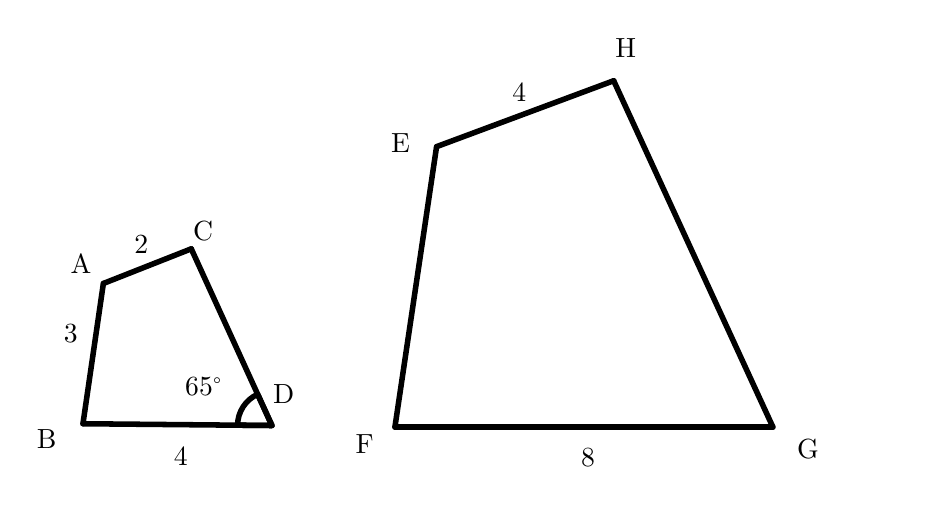
\begin{tikzpicture}[line cap=round,line join=round,>=triangle 45,x=1.0cm,y=1.0cm,scale=0.6]
\begin{scope}
\clip(-11,-2) rectangle (7,7);
\draw [shift={(-6.21808354189063,-1.4207331004506452)},line width=2.pt] (0,0) -- (114.5382925001585:0.7273722977381097) arc (114.5382925001585:179.461658965515:0.7273722977381097) -- cycle;
\draw [line width=2.pt,domain=-11:10] (-6.21808354189063,-1.4207331004506452)-- (-7.925455596547289,2.319127282722609);
\draw [line width=2.pt,domain=-11:10] (-7.925455596547289,2.319127282722609)-- (-9.786087443046851,1.5856089586218198);
\draw [line width=2.pt,domain=-11:10] (-9.786087443046851,1.5856089586218198)-- (-10.217906980189184,-1.3831503592317143);
\draw [line width=2.pt,domain=-11:10] (-10.217906980189184,-1.3831503592317143)-- (-6.21808354189063,-1.4207331004506452);
\draw [line width=2.pt,domain=-11:10] (1.0154664474060784,5.877114009247769)-- (-2.733249349834612,4.481718054144669);
\draw [line width=2.pt,domain=-11:10] (-2.733249349834612,4.481718054144669)-- (-3.6146272702343074,-1.4531933151541099);
\draw [line width=2.pt,domain=-11:10] (-3.6146272702343074,-1.4531933151541099)-- (4.385372729765693,-1.4531933151541099);
\draw [line width=2.pt,domain=-11:10] (4.385372729765693,-1.4531933151541099)-- (1.0154664474060784,5.877114009247769);
\end{scope}
\draw[color=black] (-10.258299559904163,2.0123730567025793) node {A};
\draw[color=black] (-10.985671857642274,-1.6972256617617831) node {B};
\draw[color=black] (-7.6761279029338745,2.703376739553784) node {C};
\draw[color=black] (-5.966803003249316,-0.7516416747022397) node {D};
\draw[color=black] (-8.985398038862472,2.8124825842145005) node[below] {2};
\draw[color=black] (-10.476511249225597,0.5212598463394532) node {3};
\draw[color=black] (-8.148919896463646,-1.6608570468748778) node[below] {4};
\draw[color=black] (-4.257478103564758,-1.8063315064224996) node {F};
\draw[color=black] (5.125624537256857,-1.9154373510832166) node {G};
\draw[color=black] (-3.493737190939743,4.558176098785966) node {E};
\draw[color=black] (1.270551359244876,6.558449917565769) node {H};
\draw[color=black] (-0.9843027637432642,6.049289309149092) node[below] {4};
\draw[color=black] (0.4704418317329553,-1.6972256617617831) node[below] {8};
\draw[color=black] (-8.258025741124362,-0.6061672151546177) node[right] {$65\textrm{\ensuremath{^\circ}}$};
\end{tikzpicture}

\end{multicols}

(\text{\refstepcounter{skaunta}%
\arabic{skaunta}})\hspace{2.5pt}$\angle$G の大きさを求めなさい。

\vspace{15mm}

(\text{\refstepcounter{skaunta}%
\arabic{skaunta}})\hspace{2.5pt}EF の長さを求めなさい。

\vspace{15mm}


\noindent\fbox{\large\makebox[1em]{\text{\refstepcounter{kaunta}%
\arabic{kaunta}}}} \hspace{1pt}下の図で、相似な三角形の組を見つけ、記号$\mathrel{\text{∽}}$を使って表しなさい。また、そのときに使った相似条件をいいなさい。

%
\begin{flushright}%
\footnotesize{<知・技9点>}%
\end{flushright}%


\begin{center}
\def\@captype{figure}
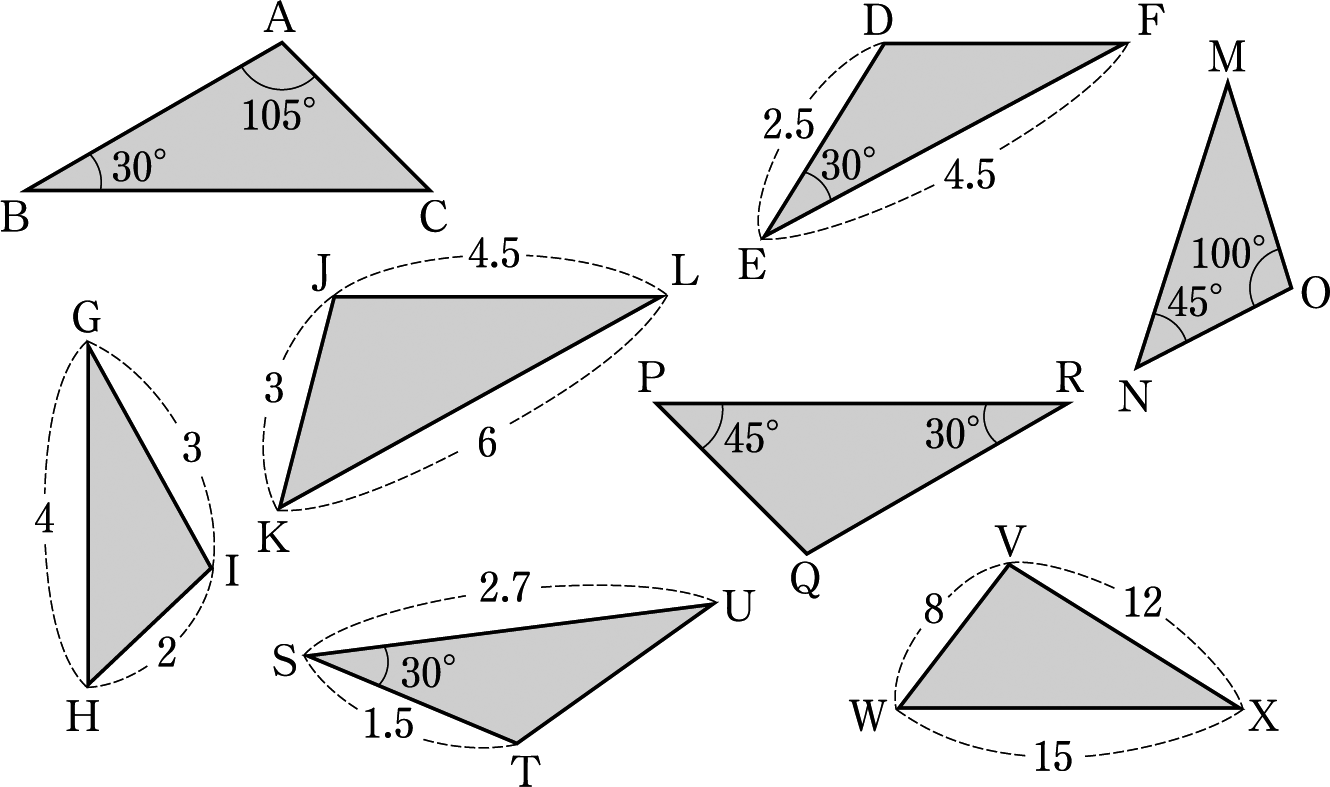
\includegraphics{image163.png}

\end{center}

\newpage

\begin{multicols}{2}
\noindent\fbox{\large\makebox[1em]{\text{\refstepcounter{kaunta}%
\arabic{kaunta}}}} \hspace{1pt}右の図で、
$$
\triangle\mbox{ABD} \mathrel{\text{∽}}\triangle\mbox{DCB}
$$
であることを証明しなさい。また、AD$/\!/$BCであることを証明しなさい。

%
\begin{flushright}%
\footnotesize{<知・技8点>}%
\end{flushright}%


\columnbreak
\begin{center}
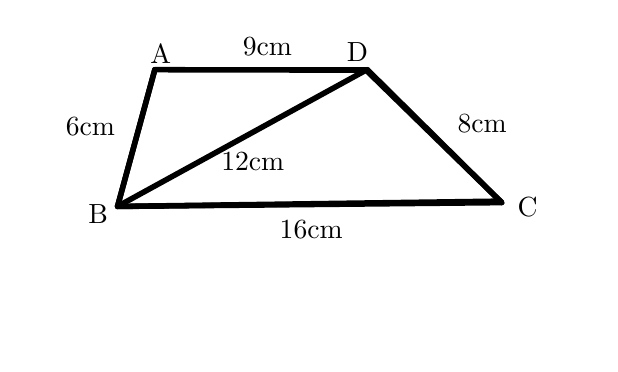
\begin{tikzpicture}[line cap=round,line join=round,>=triangle 45,x=1.0cm,y=1.0cm,scale=0.3]
\begin{scope}
\clip(-15.1316939547495,-5.989132946586327) rectangle (8.653380181286694,7.286506762253387);
\draw[line width=2.pt] (-9.749138951487486,5.631050237949681) -- (-11.327843386240136,-0.15753268947671195) -- (4.938021709324099,0.004665642304167328) -- (-0.8061679783726383,5.612592665442046) -- cycle;
\draw [line width=2.pt] (-9.749138951487486,5.631050237949681)-- (-11.327843386240136,-0.15753268947671195);
\draw [line width=2.pt] (-9.749138951487486,5.631050237949681)-- (-0.7491389514874864,5.631050237949681);
\draw [line width=2.pt] (-11.327843386240136,-0.15753268947671195)-- (-0.8061679783726383,5.612592665442046);
\draw [line width=2.pt] (-0.7491389514874864,5.631050237949681)-- (4.938021709324099,0.004665642304167328);
\draw [line width=2.pt] (-11.327843386240136,-0.15753268947671195)-- (4.670617673546776,0.06437656783772255);
\end{scope}
\draw[color=black] (-9.494558647279145,6.303869613357432) node {A};
\draw[color=black] (-12.149467534023247,-0.4606927556069892) node {B};
\draw[color=black] (-11.022040472529177,3.212537347970466) node[left] {6cm};
\draw[color=black] (-4.9848504013028645,5.8) node[above] {9cm};
\draw[color=black] (-1.1661458381777878,7.213084985530069) node[below] {D};
\draw[color=black] (-5.603116854380258,2.557902280006167) node[below] {12cm};
\draw[color=black] (5.198361767030674,0.6667343058870812) node[below right] {C};
\draw[color=black] (2.6525587249472893,3.358011807518088) node[right] {8cm};
\draw[color=black] (-3.130051042070684,-0.31521829605936724) node[below] {16cm};
\end{tikzpicture}
\end{center}
\end{multicols}
\vfill

\begin{multicols}{2}

\noindent\fbox{\large\makebox[1em]{\text{\refstepcounter{kaunta}%
\arabic{kaunta}}}} \hspace{1pt}$\triangle$ABCの辺BC, CA, ABの中点をそれぞれD, E, Fとするとき、$\triangle$DEF $\mathrel{\text{∽}}\triangle$ ABCの相似比を求めなさい。また、$\triangle$ABCの面積が$8 \si{cm}^2$のとき、$\triangle$DEFの面積を求めなさい。

%
\begin{flushright}%
\footnotesize{<知・技$3\times 2$点>}%
\end{flushright}%


\columnbreak

\def\@captype{figure}
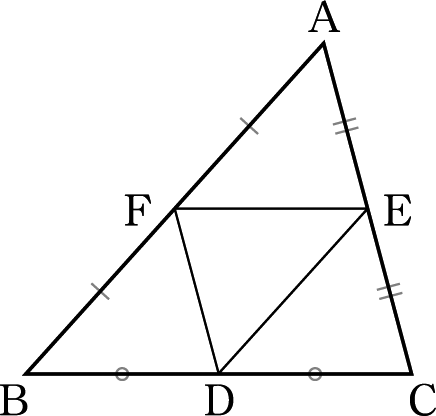
\includegraphics{image142.png}


\end{multicols}

\vfill

\setcounter{skaunta}{0}

\noindent\fbox{\large\makebox[1em]{\text{\refstepcounter{kaunta}%
\arabic{kaunta}}}} \hspace{1pt}下の図で、直線$l, m, n$が平行であるとき、$x$の値を求めなさい。

%
\begin{flushright}%
\footnotesize{<知・技$4\times 4$点>}%
\end{flushright}%


\begin{multicols}{2}
(\text{\refstepcounter{skaunta}%
\arabic{skaunta}})\hspace{2.5pt}

\def\@captype{figure}
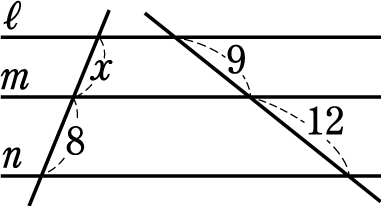
\includegraphics[width=10em]{toi1.jpg}


\columnbreak

(\text{\refstepcounter{skaunta}%
\arabic{skaunta}})\hspace{2.5pt}

\def\@captype{figure}
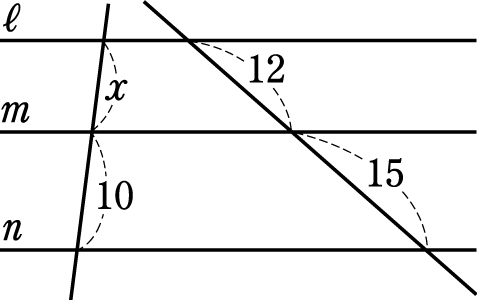
\includegraphics[width=10em]{toi2.jpg}


\end{multicols}

\vspace{15mm}

\begin{multicols}{2}

(\text{\refstepcounter{skaunta}%
\arabic{skaunta}})\hspace{2.5pt}

\def\@captype{figure}
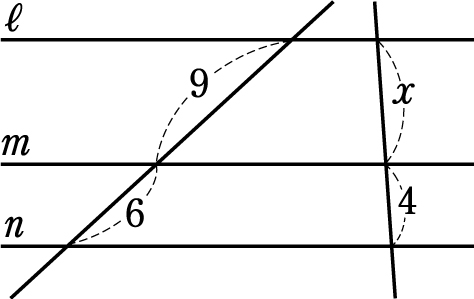
\includegraphics[width=10em]{toi3.jpg}


\columnbreak

(\text{\refstepcounter{skaunta}%
\arabic{skaunta}})\hspace{2.5pt}

\def\@captype{figure}
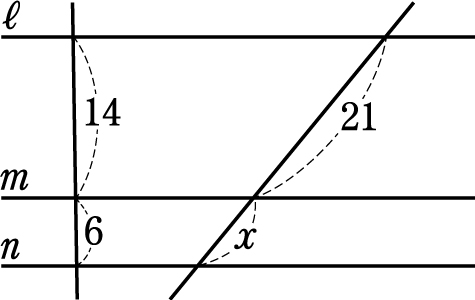
\includegraphics[width=10em]{toi4.jpg}


\end{multicols}
\vfill

\newpage

\setcounter{skaunta}{0}

\noindent\fbox{\large\makebox[1em]{\text{\refstepcounter{kaunta}%
\arabic{kaunta}}}} \hspace{1pt}下の図で、PQ$/\!/$BCとするとき、$x, \, y$の値を求めなさい。また、$\angle$Aの二等分線をADとするとき、$x$の値を求めなさい。

%
\begin{flushright}%
\footnotesize{<知・技$4\times 4$点>}%
\end{flushright}%


\begin{multicols}{2}
(\text{\refstepcounter{skaunta}%
\arabic{skaunta}})\hspace{2.5pt}

\def\@captype{figure}
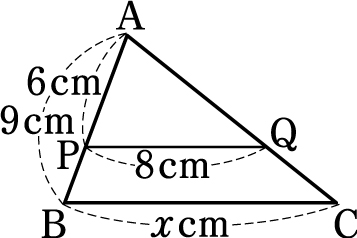
\includegraphics[width=11em]{ttoi1.jpg}


\columnbreak

(\text{\refstepcounter{skaunta}%
\arabic{skaunta}})\hspace{2.5pt}

\def\@captype{figure}
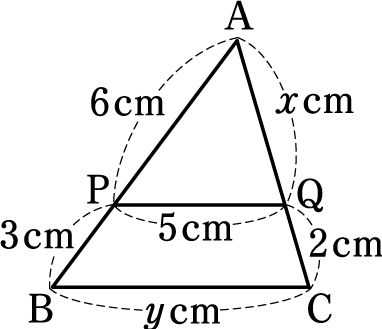
\includegraphics[width=11em]{ttoi2.jpg}

\end{multicols}

\vspace{15mm}

\begin{multicols}{2}
(\text{\refstepcounter{skaunta}%
\arabic{skaunta}})\hspace{2.5pt}

\def\@captype{figure}
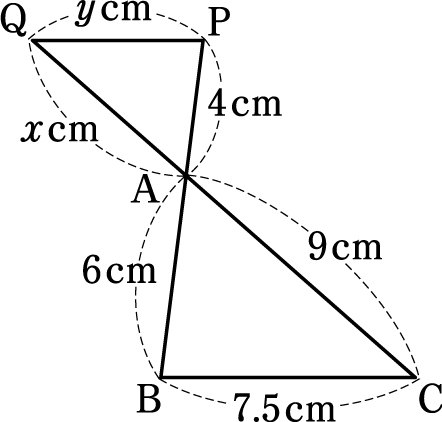
\includegraphics[width=11em]{ttoi3.jpg}


\columnbreak
(\text{\refstepcounter{skaunta}%
\arabic{skaunta}})\hspace{2.5pt}

\def\@captype{figure}
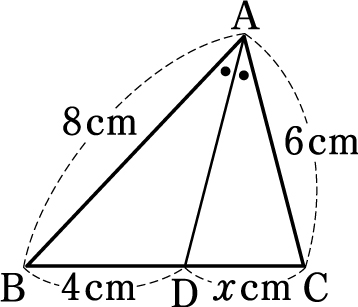
\includegraphics[width=11em]{ttoi4.jpg}


\end{multicols}

\vfill

\setcounter{skaunta}{0}
\noindent\fbox{\large\makebox[1em]{\text{\refstepcounter{kaunta}%
\arabic{kaunta}}}} \hspace{1pt}Aさんは「すべての\framebox[1.5cm][c]{\raise 0.2ex\hbox{\textcircled{\scriptsize{ア}}}}は相似であるといえるよ。」と言っています。このとき、次の問に答えなさい。

%
\begin{flushright}%
\footnotesize{<思・判・表(1)6点、(2)10点>}%
\end{flushright}%


(\text{\refstepcounter{skaunta}%
\arabic{skaunta}})\hspace{2.5pt}\framebox[1.5cm][c]{\raise 0.2ex\hbox{\textcircled{\scriptsize{ア}}}}に当てはまる平面図形を3つ答えなさい。

(\text{\refstepcounter{skaunta}%
\arabic{skaunta}})\hspace{2.5pt}\framebox[1.5cm][c]{\raise 0.2ex\hbox{\textcircled{\scriptsize{ア}}}}に当てはまらない平面図形を次のア〜エからすべて選び、それぞれについて、理由を答えなさい。ただし、テレビ画面は縦横比が$16:9$のものをいう。

ア ひし形 イ テレビ画面の長方形 ウ 二等辺三角形 エ 半円

\vfill

\newpage

\setcounter{skaunta}{0}

\begin{multicols}{2}

\noindent\fbox{\large\makebox[1em]{\text{\refstepcounter{kaunta}%
\arabic{kaunta}}}} \hspace{1pt}右の図のように、長さ$2\si{m}$の棒を地面に垂直に立てたときの影の長さが$1.7\si{m}$であった。

%
\begin{flushright}%
\footnotesize{<知・技(1)2点、(2)3点>}%
\end{flushright}%


(\text{\refstepcounter{skaunta}%
\arabic{skaunta}})\hspace{2.5pt}影の長さが$4.5\si{m}$である木の高さを求め、小数第2位を四捨五入して答えなさい。

\vspace{15mm}

(\text{\refstepcounter{skaunta}%
\arabic{skaunta}})\hspace{2.5pt}真の木の高さを$a\si{m}$として、$a$の値の範囲を不等式を使って表しなさい。



\columnbreak

\begin{center}
\def\@captype{figure}
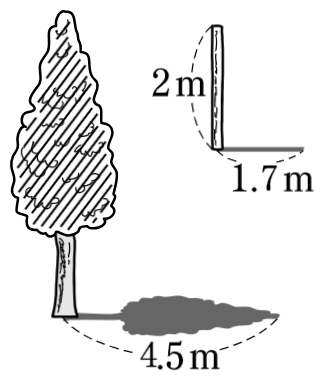
\includegraphics[height=10em]{height_wood.jpg}

\end{center}
\end{multicols}

\vspace{20mm}



\noindent\fbox{\large\makebox[1em]{\text{\refstepcounter{kaunta}%
\arabic{kaunta}}}} \hspace{1pt}$\triangle$ABCの辺BC、CA、ABの中点をそれぞれD、E、Fとし、線分FEのEを越える延長上にFE $=$ EPとなるような点Pをとる。線分ADとFPの交点をQとするとき、PE : EQ $= 2:1$であることを証明せよ。

%
\begin{flushright}%
\footnotesize{<思・判・表10点>}%
\end{flushright}%


\begin{multicols}{2}

\phantom{aaa}

\columnbreak

\begin{tikzpicture}[line cap=round,line join=round,>=triangle 45,x=1.0cm,y=1.0cm]
\clip(1.72,-6.18) rectangle (23.12,5.52);
\draw[line width=2.pt,color=black] (8.02,3.1) -- (5.24,-1.8) -- (9.82,-1.8) -- cycle;
\draw[line width=2.pt] (8.02,3.1) -- (11.21,0.65) -- (7.53,-1.8) -- cycle;
\draw [line width=2.pt,color=black] (8.02,3.1)-- (5.24,-1.8);
\draw [line width=2.pt,color=black] (5.24,-1.8)-- (9.82,-1.8);
\draw [line width=2.pt] (9.82,-1.8)-- (8.02,3.1);
\draw [line width=2.pt] (8.02,3.1)-- (7.53,-1.8);
\draw [line width=2.pt] (6.63,0.65)-- (11.21,0.65);
\draw [line width=2.pt] (8.02,3.1)-- (11.21,0.65);
\draw [line width=2.pt] (11.21,0.65)-- (7.53,-1.8);
\draw[color=black] (8.16,3.47) node {A};
\draw[color=black] (4.64,-1.51) node[below] {B};
\draw[color=black] (9.96,-1.43) node[below right] {C};
\draw[color=black] (6.4,1.13) node {F};
\draw[color=black] (9.06,0.97) node {E};
\draw[color=black] (7.54,-2.19) node {D};
\draw[color=black] (11.36,1.01) node {P};
\draw[color=black] (7.92,0.97) node[right] {Q};
\end{tikzpicture}

\end{multicols}

\vfill






















































\end{flushleft}

\end{document}
